	\section{Domain} 
		\subsection{Domainmodel}
	
		\subsection{Verknüpfungen von Task-Vorlagen und Entscheidungs-Vorlagen}
			Wissensproduzenten können Task-Vorlagen zu Entscheidungs-Vorlagen zuordnen.
			Dabei kann und soll auch eine Task-Vorlage an verschiedene Entscheidungs-Vorlagen zugeordnet werden können.
			Ebenso können Entscheidungs-Vorlagen natürlich mehrere Task-Vorlagen zugeordnet erhalten.
			
			\subsubsection{Arten der Zuordnung}
				Task-Vorlagen können mit Entscheidungs-Vorlagen auf zwei Arten verknüpft werden:
				\begin{enumerate}
					\item Sie können dann fällig werden, wenn eine Entscheidung getroffen wurde (operativer Task).
					\item Eine Task-Vorlage dient dazu, Entscheidungen zu treffen (Entscheidungstask).
				\end{enumerate}
				Auf die Task-Vorlagen selbst hat dies keinen Einfluss, sie sind unabhängig davon. 
				Ob es sich um einen operativen Task oder einen Entscheidungstask handelt hängt nur davon ab,
				ob die Task-Vorlage mit einer Entscheidung (Node) oder einer Option einer Entscheidung (Subnode) des Entscheidungsbaumes verknüpft ist.

			\subsubsection{Übertragung in \ppt}
				Aus diesen Task-Vorlagen werden beim Übertag in ein \ppt\ Tasks generiert.
				Task-Vorlagen sind generisch, da Änderungen auch alle verknüpften Entscheidungs-Vorlagen betreffen sollen.
				Aus diesem Grund werden Task-Vorlagen bei der Zuordnung verknüpft und nicht kopiert.
				
				\begin{figure}[H]
					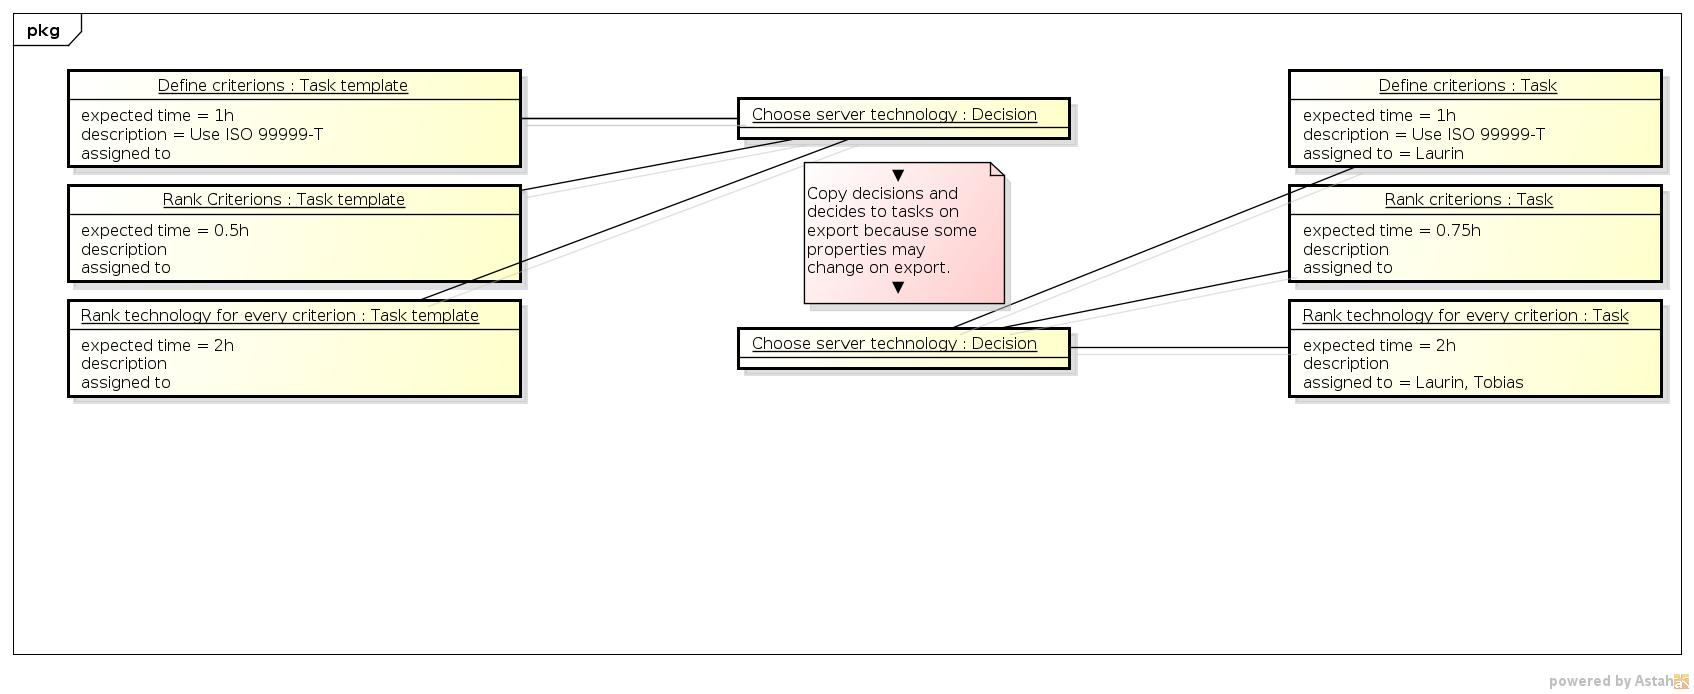
\includegraphics[width=\textwidth]{architecture/media/img/DecisionTaskRelation.jpg}
					\centering
					\caption{Übertragen von Entscheidungen und Task-Vorlagen}
					\label{fig:DecisionTaskRelation}
				\end{figure}
				
				Beim Übertragen werden aus Task-Vorlagen (konkrete) Tasks.
				Auch Entscheidungen werden zu Tasks übertragen, da \ppt's keine Entscheidungen kennen.
				Mit Entscheidungen verknüpfte Tasks werden entsprechend zu Sub-Tasks.
				
				Benutzer wollen bei der Übertragung ins \ppt\ die von der Task-Vorlage vorgegebenen Werte möglicherweise anpassen, wie z.B. den erwarteten Aufwand für den Task.
				Daher ist es sinnvoll, die Eigenschaften der Task-Vorlagen in die (konkreten) Tasks zu kopieren, anstatt sie lediglich zu verknüpfen.
				Gleiches gilt für Entscheidungen. Würde jemand im CDAR diese verändern oder Löschen, so würde dies die History zerstören.
			
		
		\subsection{EEPPI Domain}
			
				
		
		\subsection{Communication}